\section{实验三：中间人攻击与 HTTP Digest 认证分析}

\subsection{实验拓扑与服务配置}
\indent  这次实验搭建了由受害者主机（Victim）、攻击者主机（Attacker）、
网关（Gateway）以及 Web 服务器（Web Server）组成的实验环境。其中，Victim 与 Attacker 位于同一局域网中，网关负责不同网段之间的数据转发，
Web Server 则被部署于另一个子网中。
实验中主要主机的网络配置如表~\ref{tab:mitm_host} 所示，其中Gateway的MAC地址是在实验环境中获取的(和实验指导里面的不太一样)。

由于这里做的是ARP中间人攻击实验，Gateway的MAC地址没有在本次实验中被显性地使用。

\begin{table}[H]
    \centering
    \caption{ARP 中间人攻击实验主机配置}
    \label{tab:mitm_host}
    \begin{tabular}{ccc}
        \toprule
        主机 & IP 地址 & MAC 地址 \\
        \midrule
        Victim   & 192.168.26.3   & 02:ec:da:35:24:84 \\
        Attacker & 192.168.26.129 & 02:82:8a:96:0a:4c \\
        Gateway  & 192.168.26.1   & 08:00:27:d3:5c:e1  \\
        Web Server & 192.168.1.80 & 08:00:27:15:37:c5 \\
        \bottomrule
    \end{tabular}
\end{table}

实验网络拓扑如图~\ref{fig:mitm_topology} 所示。
正常情况下，Victim 发往指定外部网段的流量首先发送至默认网关
192.168.26.1，再由网关转发至 Web Server 192.168.1.80。

\begin{figure}[htbp]
    \centering
    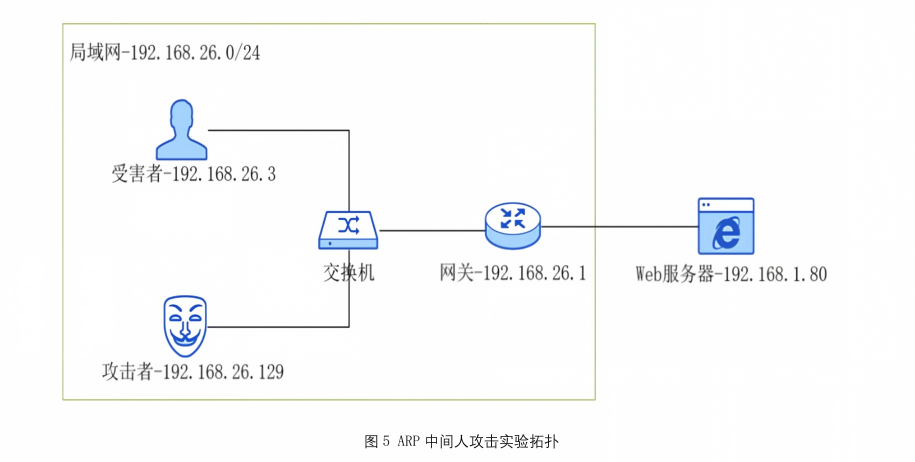
\includegraphics[width=0.75\textwidth]{figures/实验二拓扑.png}
    \caption{ARP 中间人攻击实验拓扑}
    \label{fig:mitm_topology}
\end{figure}

在实施攻击前，首先检查 Victim 主机的 ARP 缓存，
发现当前局域网内 IP 地址与 MAC 地址之间的映射关系处于正常状态。
实验结果如图~\ref{fig:arp_before} 所示。

\begin{figure}[htbp]
    \centering
    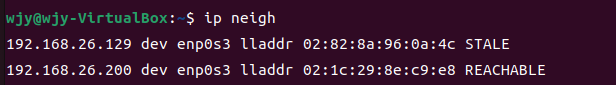
\includegraphics[width=0.75\textwidth]{figures/验证受害者的正常ARP缓存.png}
    \caption{攻击前 Victim 主机的 ARP 缓存}
    \label{fig:arp_before}
\end{figure}

由图可知，在攻击开始之前，Victim 主机维护的是正常的
IP--MAC 地址映射关系，因此可将该状态作为后续 ARP 缓存污染结果的对照。

在此之后，在Victim主机上输入
\begin{lstlisting}[language=bash]
sudo ip neigh flush all
\end{lstlisting}
清空Victim的ARP缓存。这一步是为了确保后续的 ARP 欺骗能够生效。


\subsection{ARP 缓存污染与流量捕获}

为了使 Attacker 在截获 Victim 流量后仍能够将数据继续转发至真实网关，
首先在 Attacker 主机上开启 Linux 的内核流量转发功能：

\begin{lstlisting}[language=bash]
sudo sysctl -w net.ipv4.ip_forward=1
\end{lstlisting}

开启转发后，检查参数
\texttt{net.ipv4.ip\_forward}，其值为 1，
表明 Attacker 已具备 IP 数据包转发能力。

\begin{figure}[htbp]
    \centering
    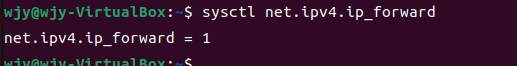
\includegraphics[width=0.72\textwidth]{figures/攻击者开启流量转发.png}
    \caption{Attacker 开启 IPv4 流量转发}
    \label{fig:ip_forward}
\end{figure}

在完成转发配置后，使用 netwox 工具实施 ARP 缓存污染。
netwox 的 80 号功能用于发送伪造的 ARP Reply。
本实验执行如下命令：

\begin{lstlisting}[language=bash]
sudo netwox 80 -e 02:82:8a:96:0a:4c -i 192.168.26.1 -E 02:ec:da:35:24:84 -I 192.168.26.3
\end{lstlisting}

其中，攻击者将自己的 MAC 地址
\texttt{02:82:8a:96:0a:4c}
伪装为网关 IP 地址 \texttt{192.168.26.1} 所对应的 MAC 地址，
并持续向 Victim 发送伪造的 ARP Reply。

\begin{figure}[htbp]
    \centering
    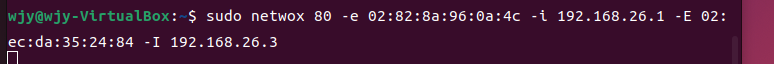
\includegraphics[width=0.85\textwidth]{figures/攻击者执行ARP欺骗.png}
    \caption{Attacker 使用 netwox 实施 ARP 缓存污染}
    \label{fig:netwox_attack}
\end{figure}

由于 ARP 协议本身缺乏有效的认证机制，
因此，即使 Victim 接收到由攻击者伪造的 ARP Reply，
也会更新其 ARP 缓存.这样一来，Victim就会将网关 IP 地址
\texttt{192.168.26.1}错误地映射到 Attacker 的 MAC 地址\texttt{02:82:8a:96:0a:4c}。

此后，Victim 仍然认为自己正在向真实网关发送数据，
但其流量实际上会首先被劫持至 Attacker。
Attacker 再利用已经开启的内核转发功能将数据包转交给真实网关，
从而使流量经过中间人。

为了验证在 ARP 缓存污染之后 Victim 的正常通信没有被破坏，
在 Victim 上向 Web Server 192.168.1.80 发送 ICMP Echo Request：

\begin{lstlisting}[language=bash]
ping -c 4 192.168.1.80
\end{lstlisting}

实验结果如图~\ref{fig:ping_server} 所示。
\begin{figure}[htbp]
    \centering
    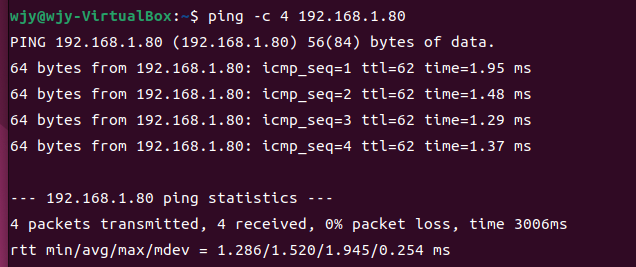
\includegraphics[width=0.80\textwidth]{figures/受害者ARP污染后的通行.png}
    \caption{ARP 缓存污染后 Victim 与 Web Server 的连通性}
    \label{fig:ping_server}
\end{figure}

实验中共发送 4 个 ICMP 请求，并全部收到响应，
丢包率为 0\%。
该结果说明在 Attacker 成为中间节点后，
其仍能够正常转发 Victim 的网络流量，
因此 ARP 中间人攻击没有直接导致 Victim 网络连接中断。

为了进一步验证 Victim 的数据流量已经能够被 Attacker 捕获，
在 Attacker 的 \texttt{enp0s3} 网卡上使用 tcpdump 对
ARP 和 ICMP 数据包进行监听：

\begin{lstlisting}[language=bash]
sudo tcpdump -n -e -i enp0s3 'arp or icmp'
\end{lstlisting}

抓包结果如图~\ref{fig:tcpdump_mitm} 所示。

\begin{figure}[htbp]
    \centering
    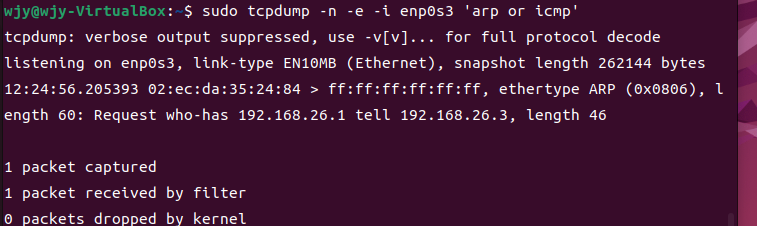
\includegraphics[width=0.88\textwidth]{figures/攻击者截获流量.png}
    \caption{Attacker 捕获 Victim 产生的网络流量}
    \label{fig:tcpdump_mitm}
\end{figure}

从抓包结果可以看到来自 Victim
（MAC 地址为 \texttt{02:ec:da:35:24:84}）
的数据帧已经能够被 Attacker 捕获。
结合 Victim ARP 缓存中网关 IP 与 Attacker MAC 的错误映射，
可以确认 ARP 缓存污染已经生效，
Attacker 确实位于 Victim 与真实网关之间的流量转发路径上。


\subsection{认证数据分析与离线验证}

在完成 ARP 中间人攻击后，在 Victim 浏览器中访问：

\begin{center}
\texttt{http://192.168.1.80}
\end{center}
输入登录的用户名与密码，如图\ref{fig:access_http}所示，可见密码为 \texttt{123456}。

\begin{figure}[htbp]
    \centering
    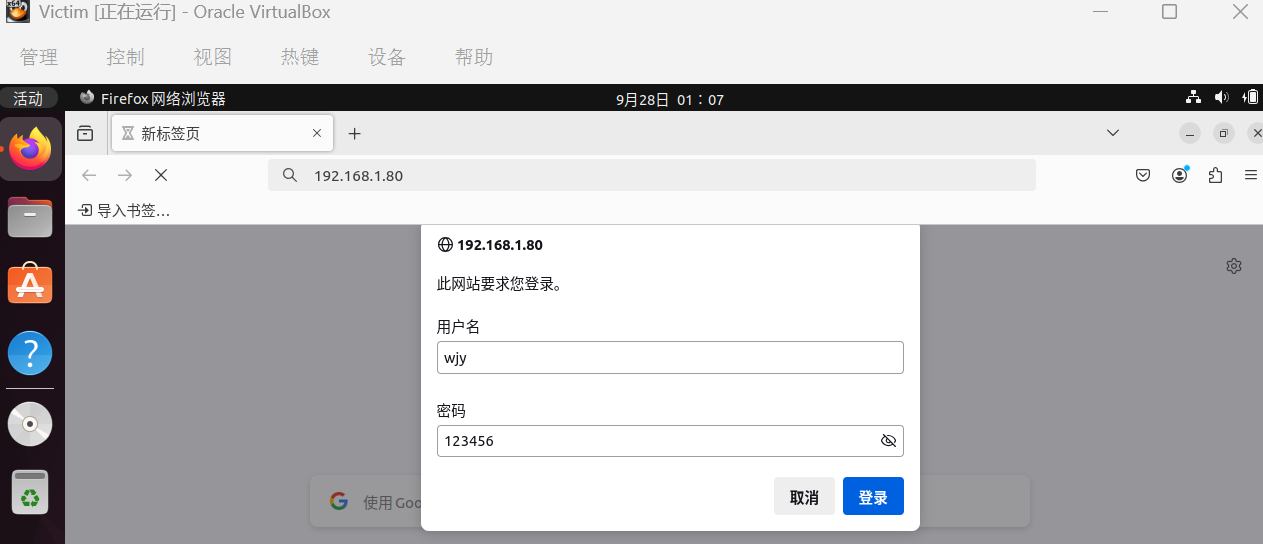
\includegraphics[width=0.92\textwidth]{figures/访问相应网站.png}
    \caption{Victim 访问相应网站的登录页面}
    \label{fig:access_http}
\end{figure}

同时在 Attacker 上启动 Wireshark，
监听 Victim 与 Web Server 之间的 HTTP 通信。
当 Victim 提交 HTTP Digest 认证信息后，
Attacker 可以在捕获到的 HTTP 请求中观察到
\texttt{Authorization: Digest} 字段。

\begin{figure}[htbp]
    \centering
    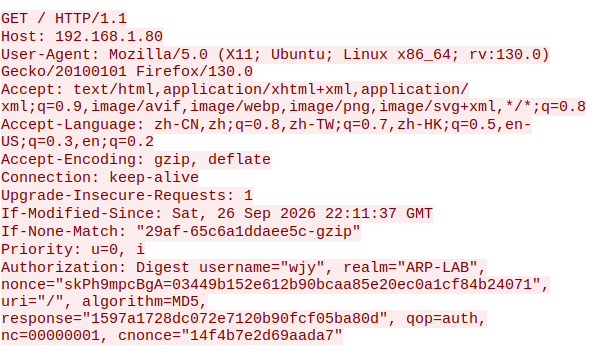
\includegraphics[width=0.92\textwidth]{figures/WireShark截获流量.png}
    \caption{Wireshark 捕获的 HTTP Digest 认证信息}
    \label{fig:digest_packet}
\end{figure}

从捕获的数据包中提取到的主要 Digest 参数如
表~\ref{tab:digest_params} 所示。

\begin{table}[htbp]
    \centering
    \caption{捕获的 HTTP Digest 认证参数}
    \label{tab:digest_params}
    \begin{tabular}{cl}
        \toprule
        参数 & 实验值 \\
        \midrule
        username & \texttt{wjy} \\
        realm & \texttt{ARP-LAB} \\
        method & \texttt{GET} \\
        uri & \texttt{/} \\
        nonce &
        \texttt{skPh9mpcBgA=03449b152e612b90bcaa85e20ec0a1cf84b24071} \\
        nc & \texttt{00000001} \\
        cnonce & \texttt{14f4b7e2d69aada7} \\
        qop & \texttt{auth} \\
        response & \texttt{1597a1728dc072e7120b90fcf05ba80d} \\
        \bottomrule
    \end{tabular}
\end{table}

HTTP Digest 认证不会直接在网络中传输用户口令，
而是使用用户名、realm、口令以及服务器和客户端提供的随机参数
共同计算认证摘要。

对于本实验采用的 \texttt{qop=auth} 情况，
首先计算：

\[
HA_1 =
MD5(
username : realm : password
)
\]

以及：

\[
HA_2 =
MD5(
method : uri
)
\]

最终客户端发送的认证摘要为：

\[
response =
MD5(
HA_1 : nonce : nc : cnonce : qop : HA_2
)
\]

因此，虽然攻击者无法直接从网络数据包中读取明文密码，
但是在已知 username、realm、nonce、nc、cnonce、
qop、method、uri 和 response 的情况下，
可以针对候选密码重新计算 Digest，
并将计算结果与捕获到的 response 进行比较。


根据上述原理，本实验编写 Python 程序\texttt{digest\_crack.py}对候选口令进行离线验证。
核心验证过程如下：

\begin{lstlisting}[language=Python]
import hashlib


# Wireshark 中提取的 Digest 参数
username = "wjy"
realm = "ARP-LAB"
method = "GET"
uri = "/"

nonce = "skPh9mpcBgA=03449b152e612b90bcaa85e20ec0a1cf84b24071"
nc = "00000001"
cnonce = "14f4b7e2d69aada7"
qop = "auth"

response = "1597a1728dc072e7120b90fcf05ba80d"


# 计算 MD5
def compute_md5_hash(text):
    return hashlib.md5(text.encode("utf-8")).hexdigest()


# 定义 MD5 碰撞函数
def MD5Collision(response, dictfilepath):

    # 打开字典文件，读取所有口令
    with open(dictfilepath, "r") as file:
        passwords = file.readlines()

    # 计算 MD5 摘要，与 response 进行碰撞
    for password in passwords:
        password = password.strip()

        # 构建 A1 和 A2
        textpart_A1 = f"{username}:{realm}:{password}"
        textpart_A2 = f"{method}:{uri}"

        A1_MD5 = compute_md5_hash(textpart_A1)
        A2_MD5 = compute_md5_hash(textpart_A2)

        # 构建最终 Digest 输入
        textpart = (
            f"{A1_MD5}:{nonce}:{nc}:{cnonce}:{qop}:{A2_MD5}"
        )

        # 计算密码的 MD5 摘要
        digest = hashlib.md5(
            textpart.encode("utf-8")
        ).hexdigest()

        # 检查摘要是否与捕获到的 response 匹配
        if digest == response:
            print(f"口令正确 : {password}")
            return password

    print("Password not found in dictionary.")
    return None


# 使用六位数字密码本
MD5Collision(response, "Password.txt")
\end{lstlisting}

实验使用由六位数字组成的候选密码集合
\texttt{Password.txt}。
程序依次读取候选口令，根据捕获到的 Digest 参数重新计算
\texttt{response}，若计算结果与 Wireshark 捕获到的
\texttt{response} 完全相同，则说明当前候选口令与认证时使用的口令一致。

运行程序\texttt{digest\_crack.py}后，成功找到了能够产生相同 Digest 响应值的六位数字口令，
实验结果如图~\ref{fig:digest\_crack} 所示。

\begin{figure}[htbp]
    \centering
    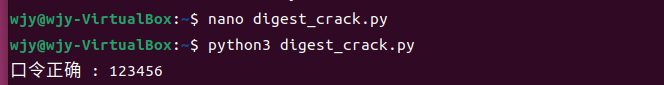
\includegraphics[width=0.75\textwidth]{figures/得出口令.png}
    \caption{HTTP Digest 认证口令离线验证结果}
    \label{fig:digest\_crack}
\end{figure}


程序输出的候选口令与 Victim 实际登录时使用的口令一致，
说明根据中间人攻击过程中捕获的 HTTP Digest 参数，
可以在已知较小口令空间的条件下完成离线口令验证。


\subsection{结果与分析}

实验二完成了基于 ARP 缓存污染的中间人攻击。
攻击前，Victim 的 ARP 缓存中保存正常的 IP--MAC 地址映射；
攻击过程中，Attacker 持续向 Victim 发送伪造的 ARP Reply，
使 Victim 将网关 IP 地址错误地映射到 Attacker 的 MAC 地址。
因此，Victim 原本应直接发送给真实网关的流量首先到达 Attacker。

与此同时，在 Attacker 主机开启 IP 转发后，
Attacker 能够继续将截获的流量转发至真实网关，
因此 Victim 与 Web Server 之间的网络通信并未中断。
供给的关键在于：
Victim 无法仅通过通信正常来直接判断流量有没有经过中间节点Attacker，
这体现了 ARP 中间人攻击所具有的隐蔽性。

通过 Wireshark 抓包可以进一步观察到 Victim 与 Web Server
之间的 HTTP Digest 认证流量。
Digest 认证不会直接传输用户的明文口令，
网络中传输的是由口令及 nonce、cnonce、nc、qop 等参数共同计算得到的摘要。
因此，与直接传输明文口令相比，
Digest 认证能够避免口令直接暴露在网络中。

然而，本实验同时表明，攻击者一旦能够截获完整的 Digest 认证参数，
仍然可以针对候选口令进行离线计算。
由于本实验限定的是六位纯数字密码，
密钥候选空间较小，因此可以枚举候选口令，
重新计算 Digest 并与捕获到的 response 进行比较，
最终验证出正确口令。

综上，实验验证了 ARP 协议缺乏身份认证所带来的安全风险。
攻击者能够通过伪造 ARP 映射进入正常流量的转发路径，
进一步监听上层协议产生的网络流量。

